\section{Laboratory work implementation}

\subsection{Tasks and Points}

Basic Level:

    - Create a Windows application what will display a dialogue box on some event (ex. on clicking some button)
    
    - Add a system menu to your application with at least 3 items (add actions to that items)
   
    - Hook keyboard input. Add 2 custom events for 2 different keyboard combinations


Normal Level:

    - Realize the tasks from Basic Level.

    - Add a scroll bar that will change any visible parameter of any other element 


Advanced Level:

	- Realize the tasks from Normal Level
	- Customize your application by adding an icon and using different cursor in application

Bonus Point:
	
	- Use a scroll bar to scroll through application working space. Scroll should appear only when necessary

\subsection{Laboratory work analysis}

Repository:

https://github.com/VictorIstratii151/WP-labs

\subsection{Proving my work}

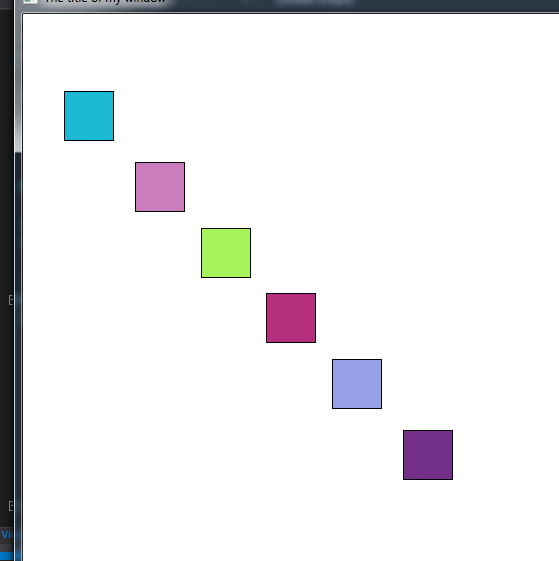
\includegraphics{im1}
My window application has 2 dialogues. One of them is a permanent child window of the original application



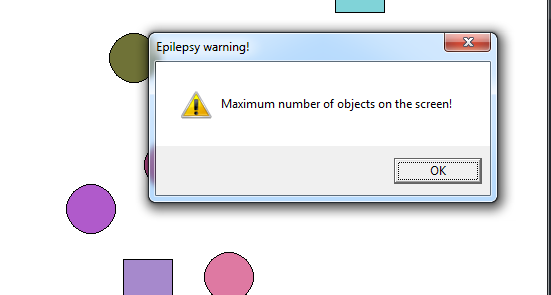
\includegraphics{im3}
The second is displayed when the user clicks the button 'Hi'



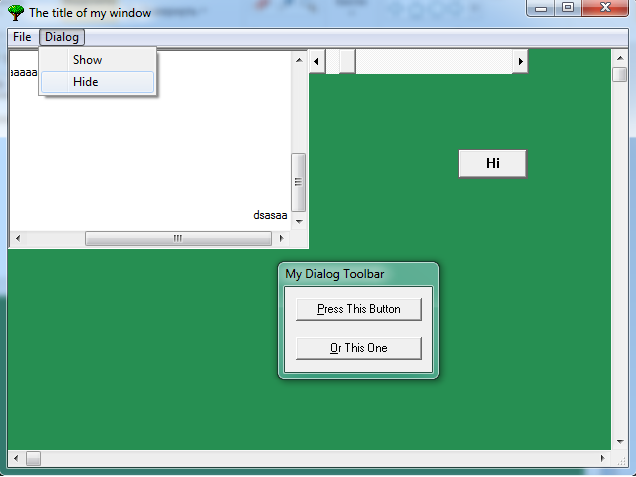
\includegraphics{im6}
Also my window contains a menu in the non-client area with 3 actions: 

- 'File' allows to exit the program
- 'Dialogue' allows to hide or show the dialog box which is present from start



The keyboard hooks in my program are represented by 3 combinations:
- 'ctrl' + 'x' to close the window
- 'ctrl' + 'm' to minimize the window
- 'ctrl' + 'r" to restore the window



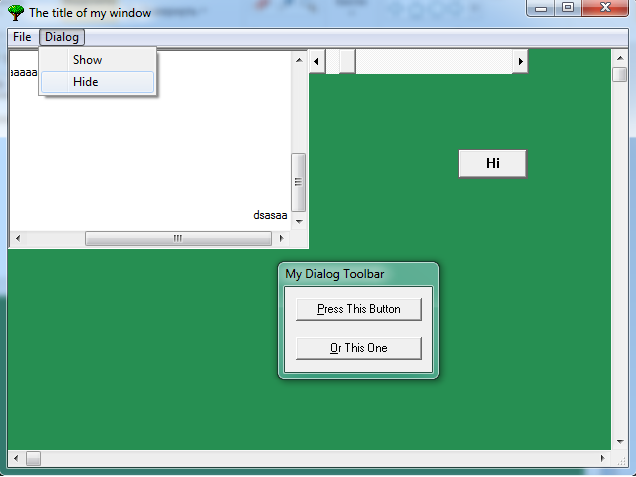
\includegraphics{im6}
In my window is present a custom scroll bar control, which allows changing the background color to random values. It is possible to do such a thing not only by dragging the scroll thumb, but also by clicking on the arrow buttons and on the area between arrows and thumb:


As it can be seen from all the screen shots, I've added an icon for the window, which is displayed on the title box and also is represented on the miniature of program in the task bar.
I've also added a custom cursor for this program. However it is not seen due to the fact that the cursor is not displayed on screen shots.



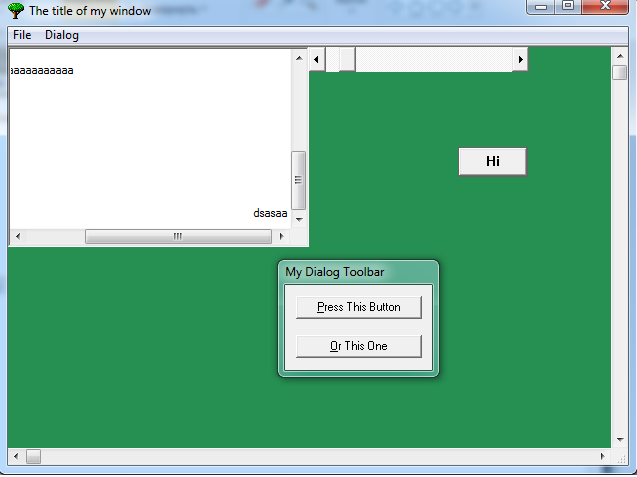
\includegraphics{im5}
To complete the bonus point I have created an edit control, where can be written text. Because the edit section has a stable size, when it is written too much text, automatically appear the requested thumbs for scrolling. Also the scroll thumb is decreasing in size when it is written more and more text:

\clearpage